%!TEX root = ../talk.tex

\section{Comparison}\label{sec:numer}

%%%
\subsection{Speed}
%%%

%%%
\subsection{Scalability}
%%%

\begin{frame}
  \MyLogo
  \frametitle{Numerical tests}  
		\begin{itemize}
		\item Neural networks and data sets:
		For synthetic data testing, a large neural network(FCN-S) with around 55 million parameters is used to evaluate the performance of FCN; and we choose the classical AlexNet(AlexNet-S) as representatives of CNNs. For real-world data experiments, a smaller FCN(FCN-R) is constructed for MNIST data set; an AlexNet(AlexNet-R) architecture is used for Cifar10 data set. For RNNs,considering that the main computation complexity is related to the length of inputsequence, we select 2 LSTM layers for testing, with input length of 32.
		\end{itemize}
		\begin{figure}[htbp] 
			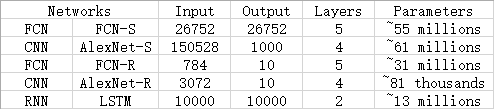
\includegraphics[height=0.9in]{figures/models.png} 
			\caption{The experimental setup of neural networks for synthetic data and real data}
		\end{figure}
	
\end{frame}

%

\begin{frame}
	\MyLogo
	\frametitle{Numerical tests}  
	\begin{itemize}
		\item Hardware platforms: We use two types of multi-core
		CPUs, one quad-core desktop CPU (i.e., Intel i7-3820 CPU
		@ 3.60GHz) and two 8-core server-grade CPUs (i.e., Intel
		Xeon CPU E5-2630 v3 @ 2.40GHz), to test the performance of tools with different number of threads; and two
		generations of GPU cards, GTX 1080 @ 1607MHz with
		Pascal architecture, and Telsa K80 @ 562MHz with Kepler
		architecture, are used to compare the performance on accelerators. 
	\end{itemize}
	
	\begin{figure}[htbp] 
		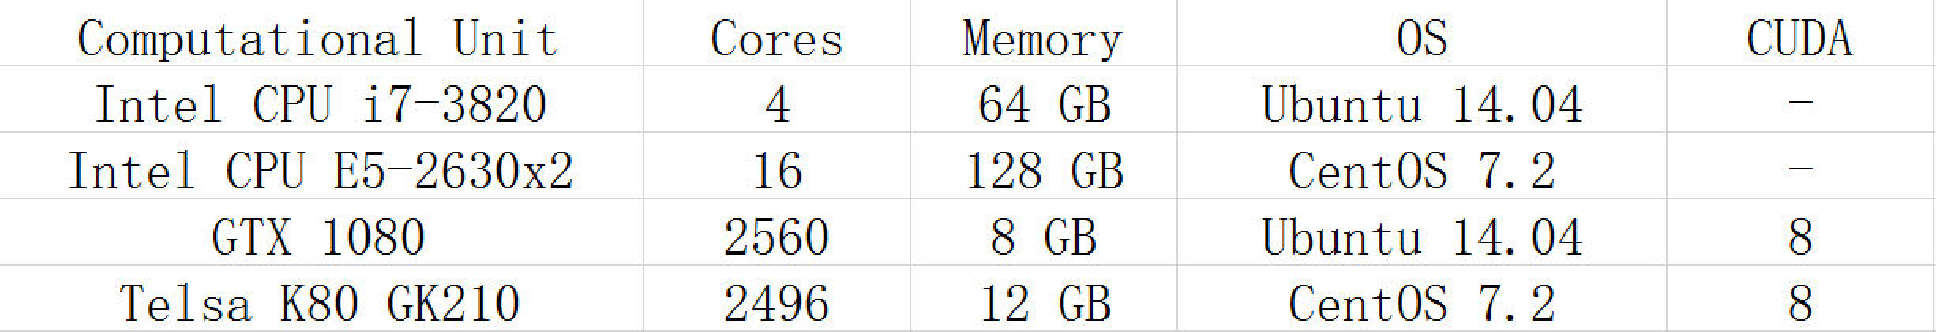
\includegraphics[height=1in]{figures/platforms.pdf} 
		\caption{The experimental hardware setting for data parallelization}
	\end{figure}
	
\end{frame}

%

\begin{frame}
	\MyLogo
	\frametitle{Numerical tests}  
	\begin{itemize}
		\item Numerical test results:
	\end{itemize}
	\begin{figure}[htbp] 
		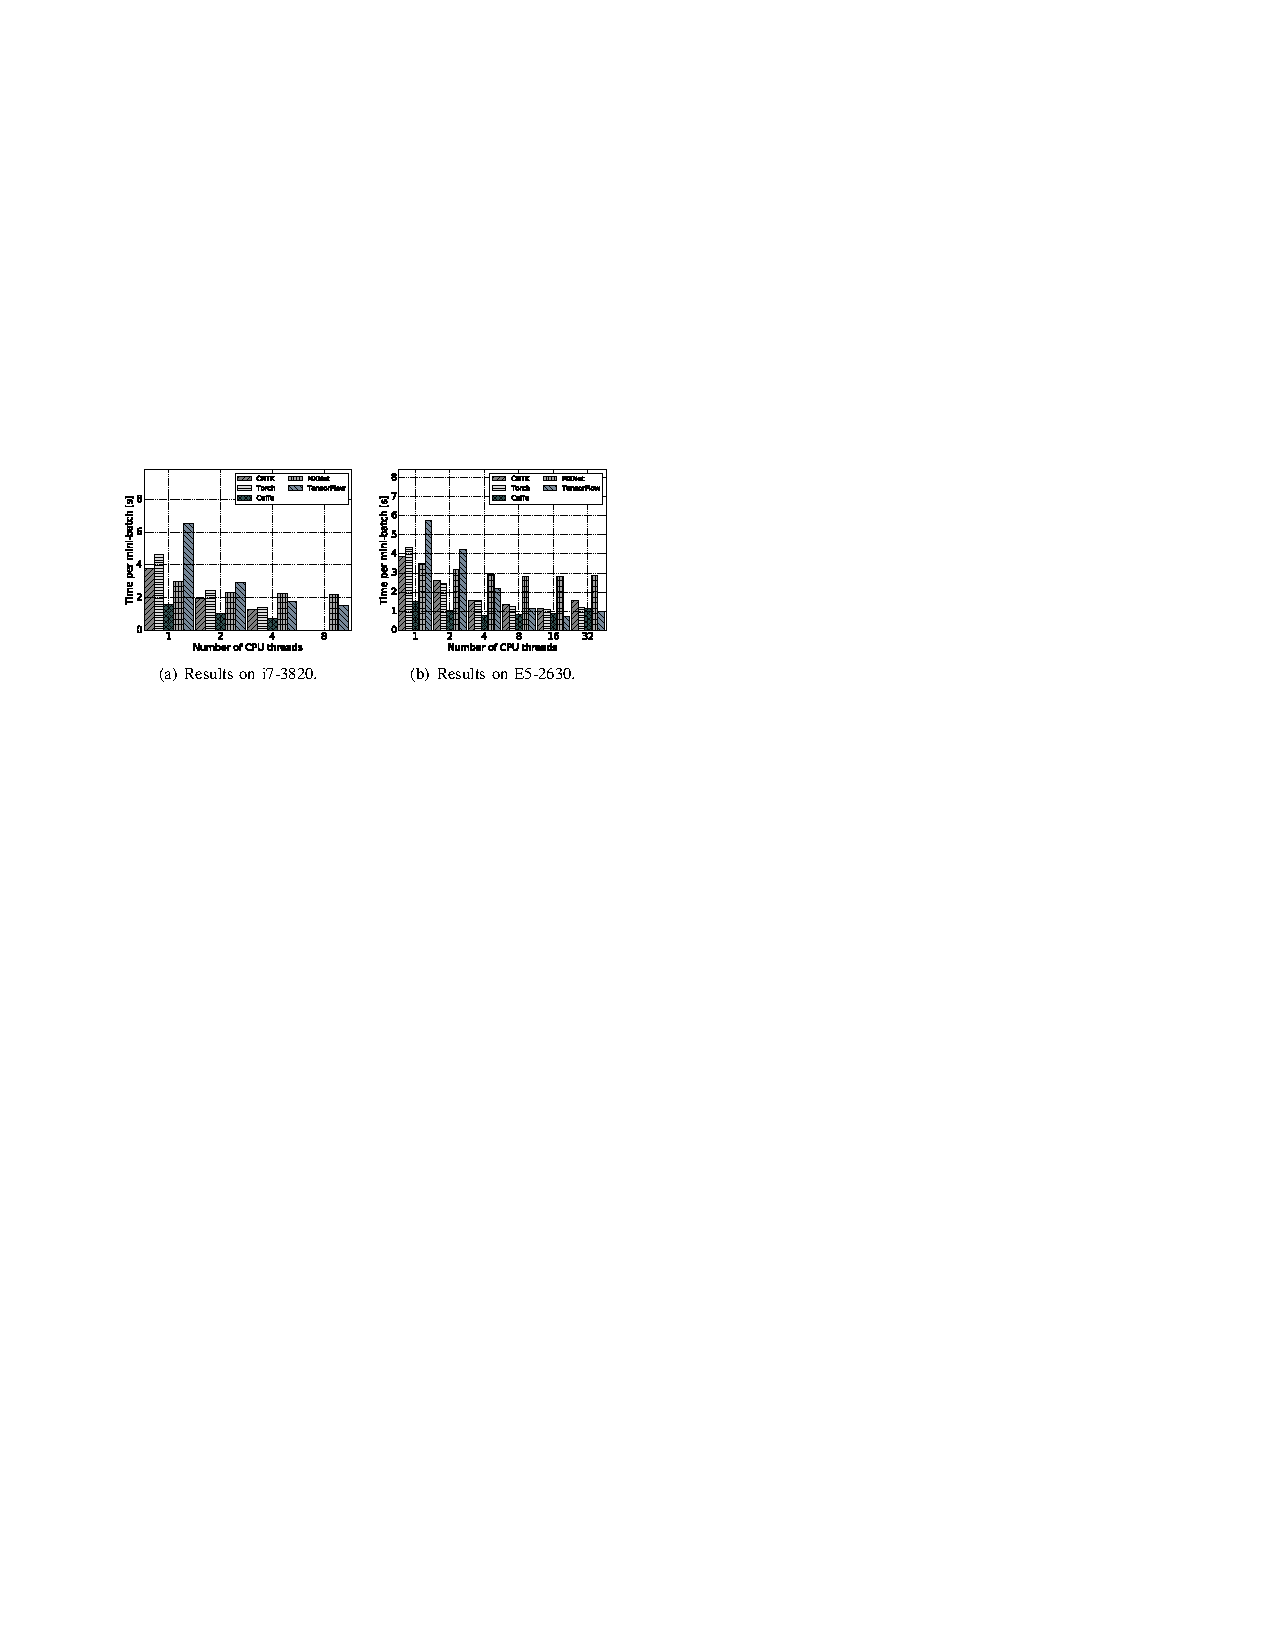
\includegraphics[height=1.8in]{figures/AlexNet-S1.pdf} 
		\caption{AlexNet-S performance comparison on CPU platform with a mini-batch size of 16.(The lower the better.)}
	\end{figure}	
\end{frame}

%

\begin{frame}
	\MyLogo
	\frametitle{Numerical tests}  
	\begin{figure}[htbp] 
		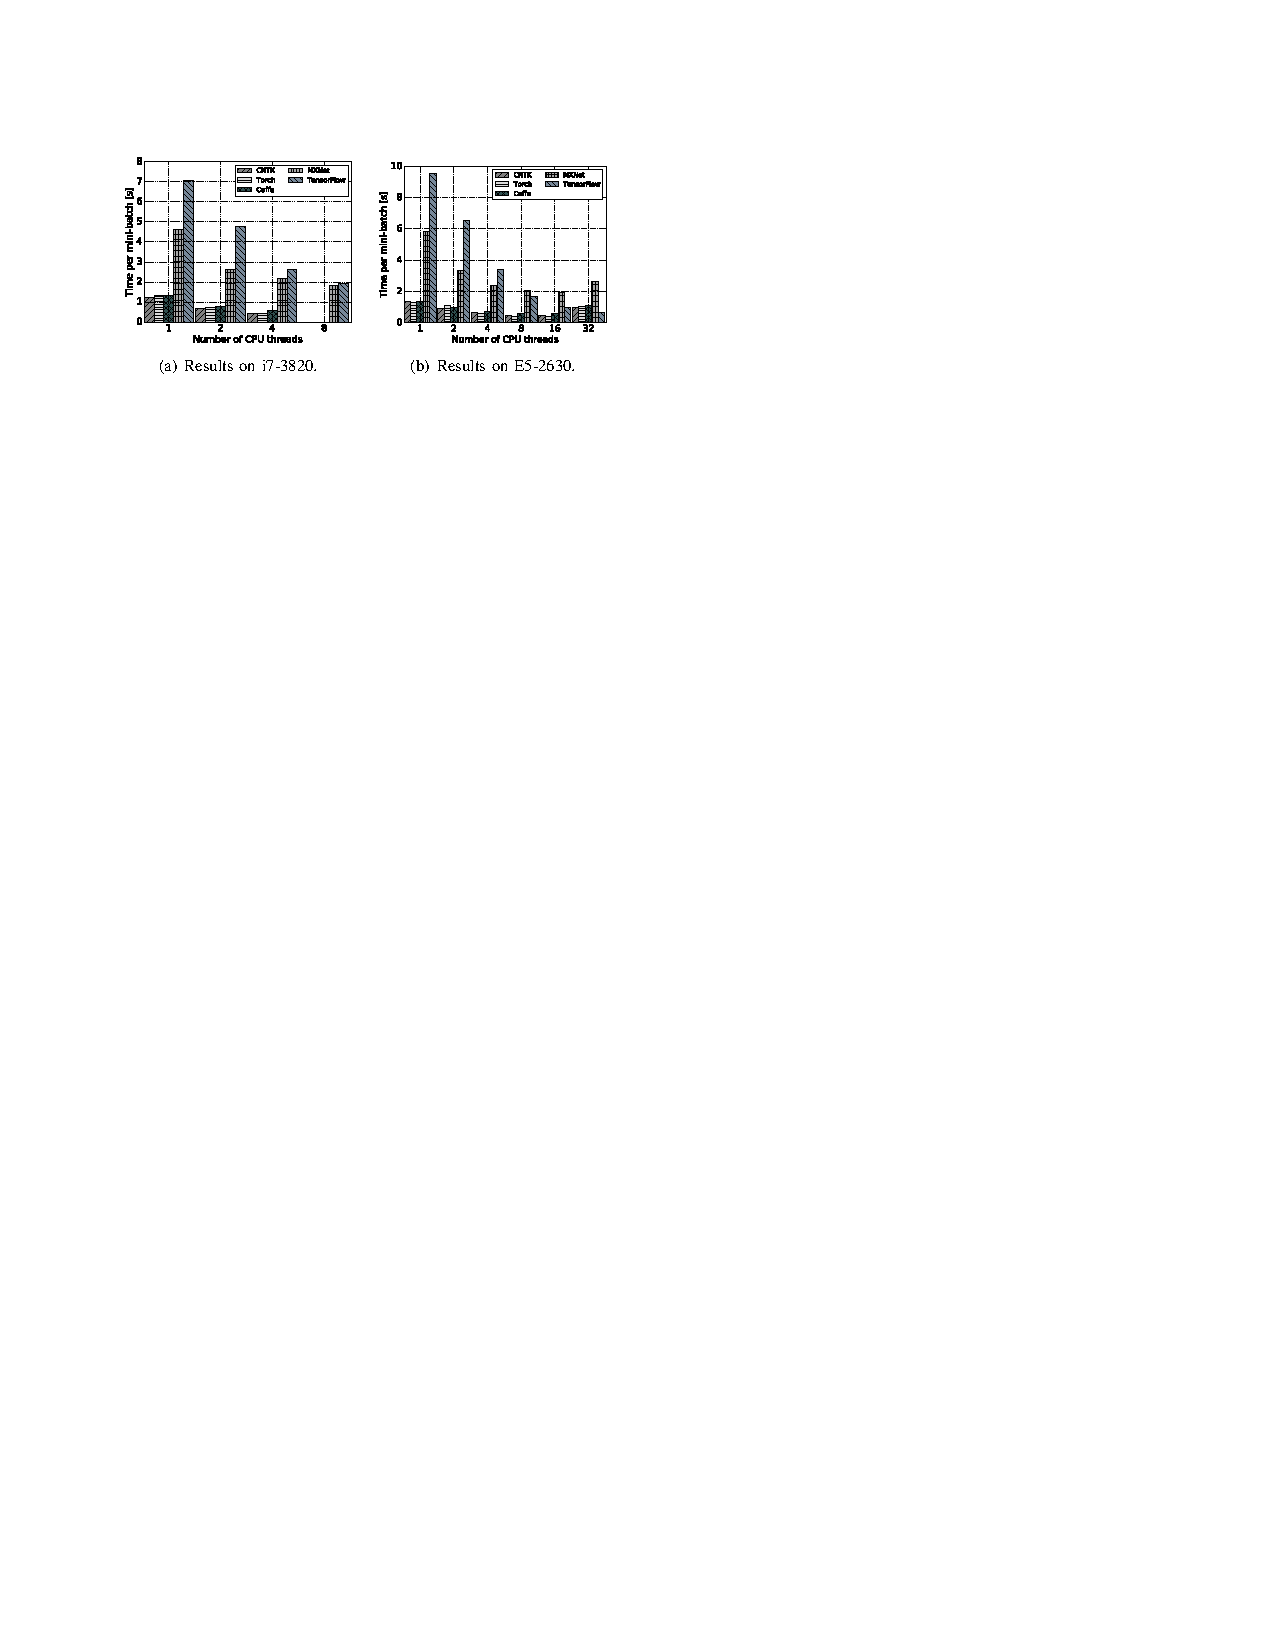
\includegraphics[height=1.8in]{figures/FCN-S1.pdf} 
		\caption{FCN-S performence comparison on CPU platform with a mini-batch size of 64.(The lower the better.)}
	\end{figure}
\end{frame}
%

\begin{frame}
	\MyLogo
	\frametitle{Numerical tests}  
	\begin{figure}[htbp] 
		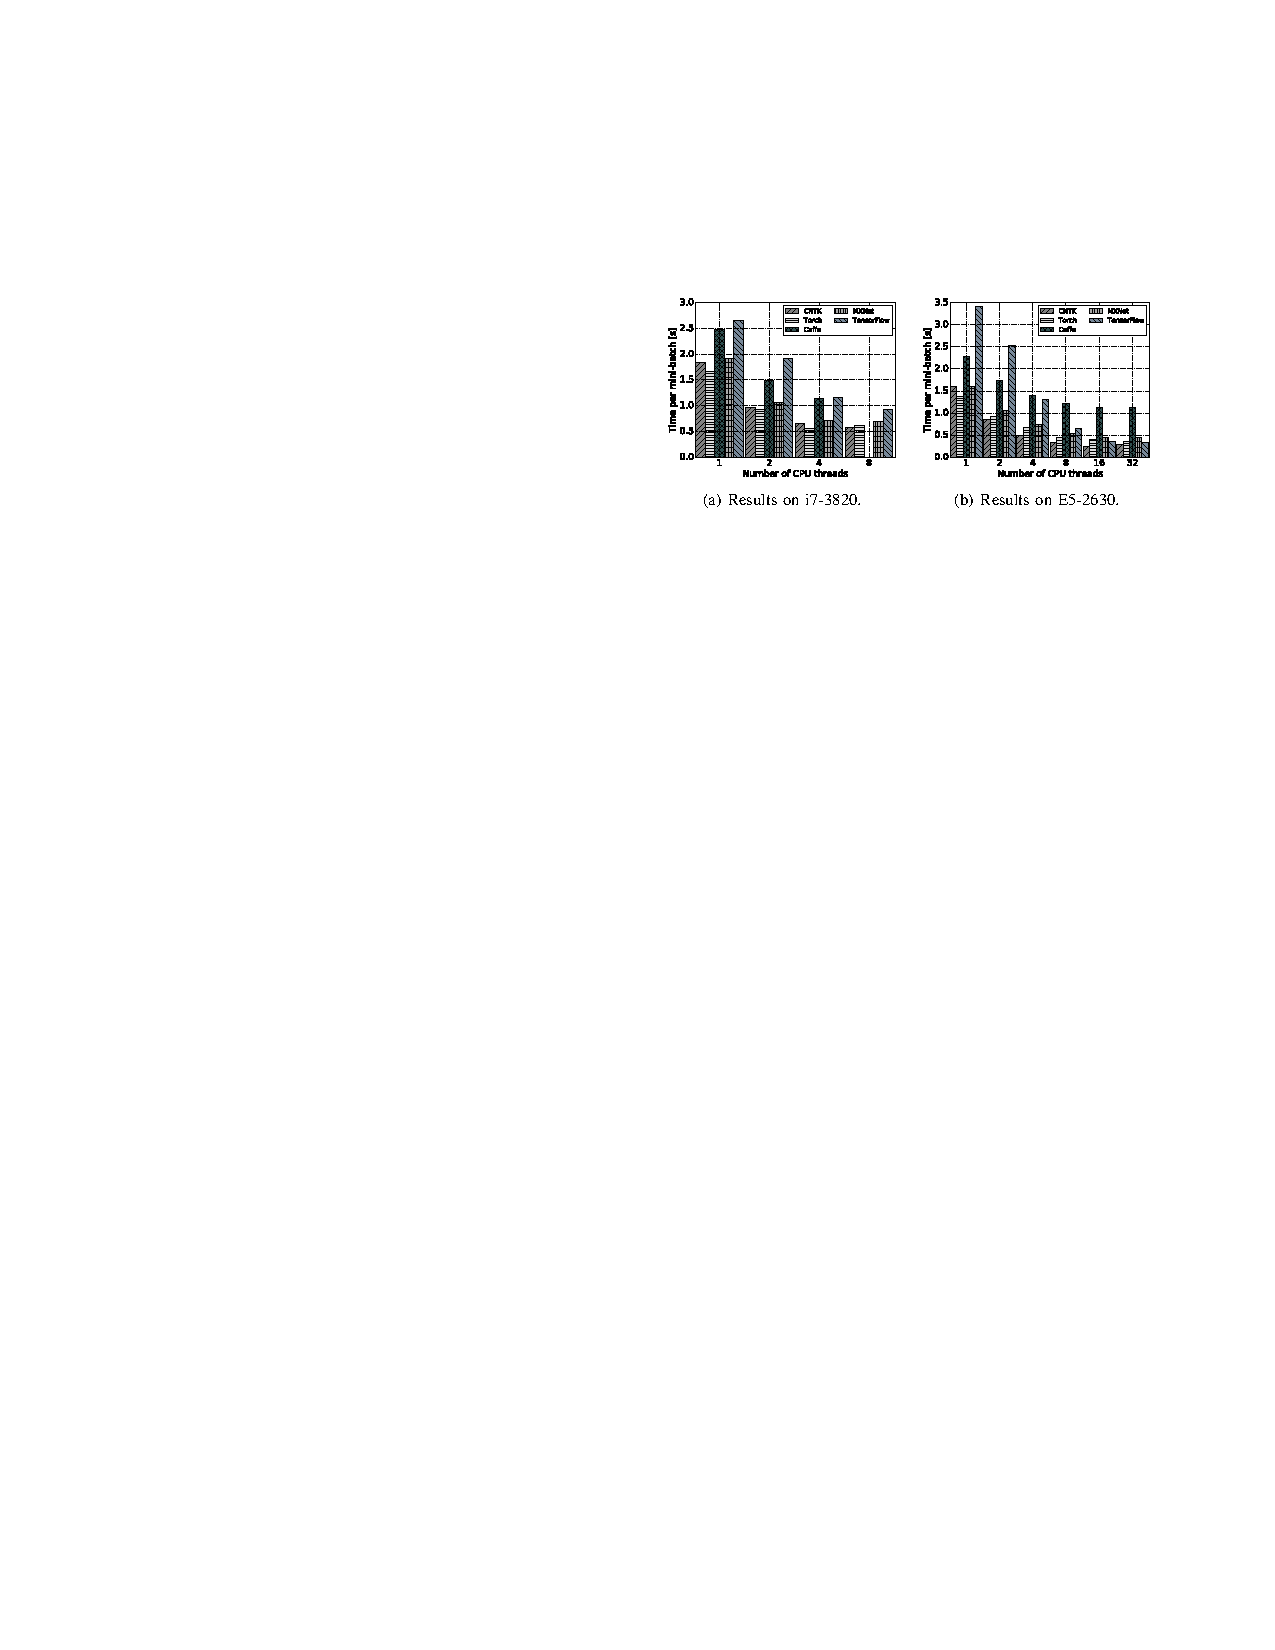
\includegraphics[height=1.8in]{figures/FCN-R1.pdf} 
		\caption{The FCN-R performance comparison on CPU platform with a mini-batch size of 1024.(The lower the better.)}
	\end{figure}
\end{frame}
%

\begin{frame}
	\MyLogo
	\frametitle{Numerical tests}  
	\begin{figure}[htbp] 
		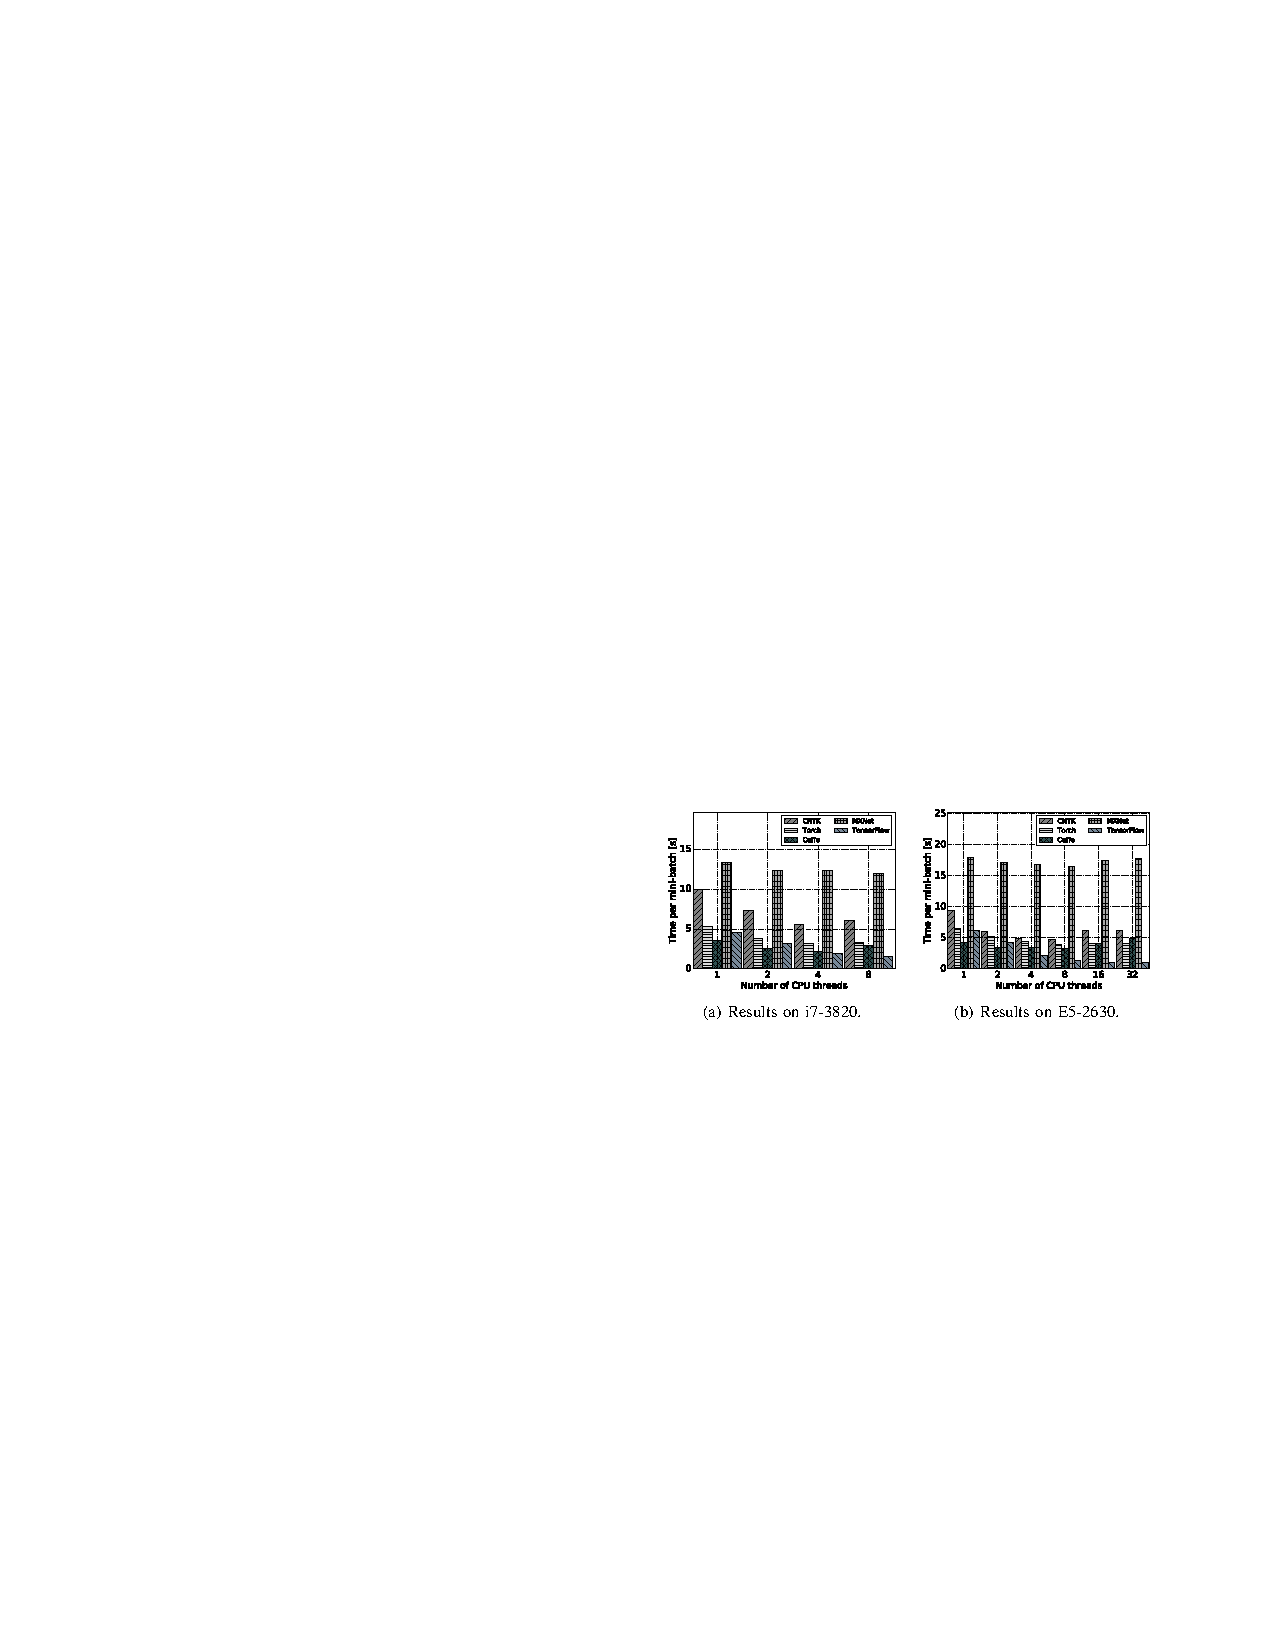
\includegraphics[height=1.8in]{figures/AlexNet-R1.pdf} 
		\caption{AlexNet-R performance comparison on CPU platform with a mini-batch size of 1024.(The lower the better.)}
	\end{figure}
\end{frame}
%

\begin{frame}
	\MyLogo
	\frametitle{Numerical tests}  
	\begin{figure}[htbp] 
		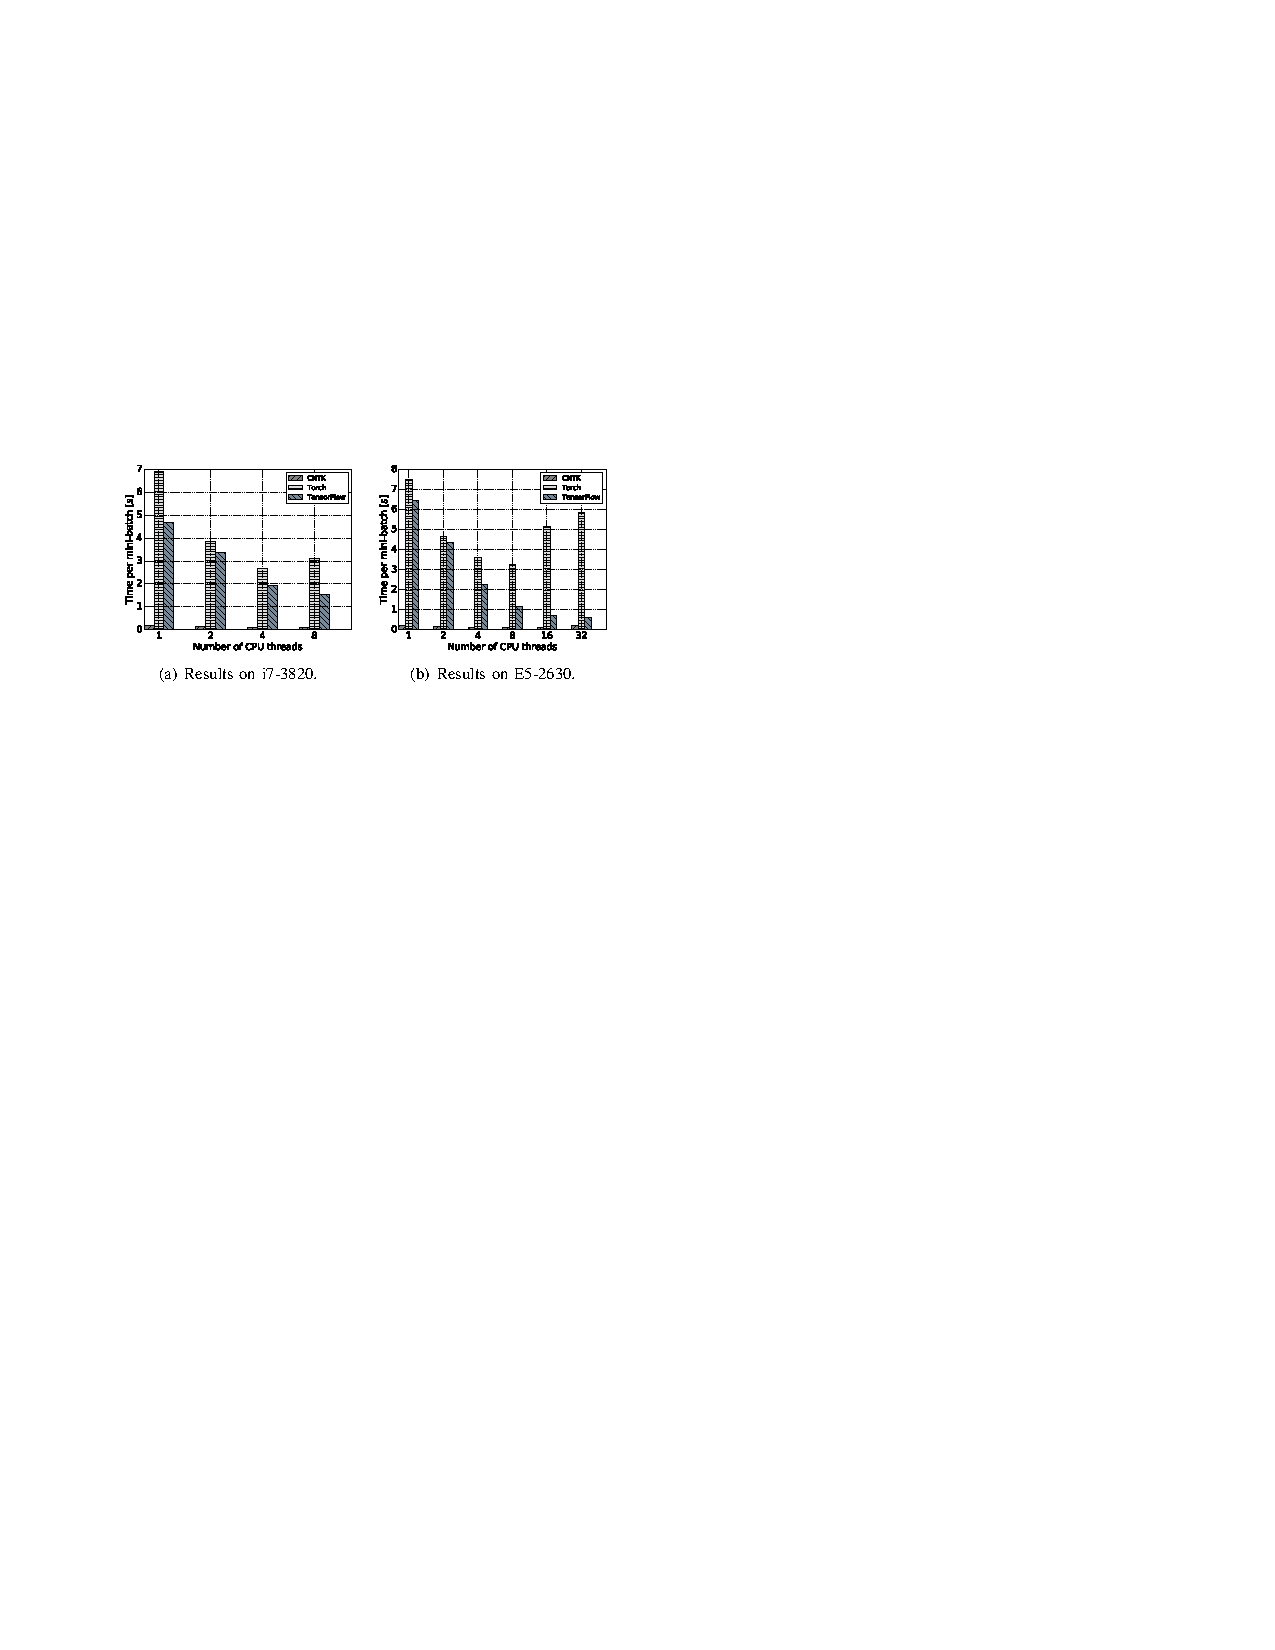
\includegraphics[height=1.8in]{figures/LSTM1.pdf} 
		\caption{LSTM performance comparison on CPU platform with a mini-batch size of 256.(The lower the better.)}
	\end{figure}
\end{frame}

%

\begin{frame}
	\MyLogo
	\frametitle{Numerical tests}  
	\begin{figure}[htbp] 
		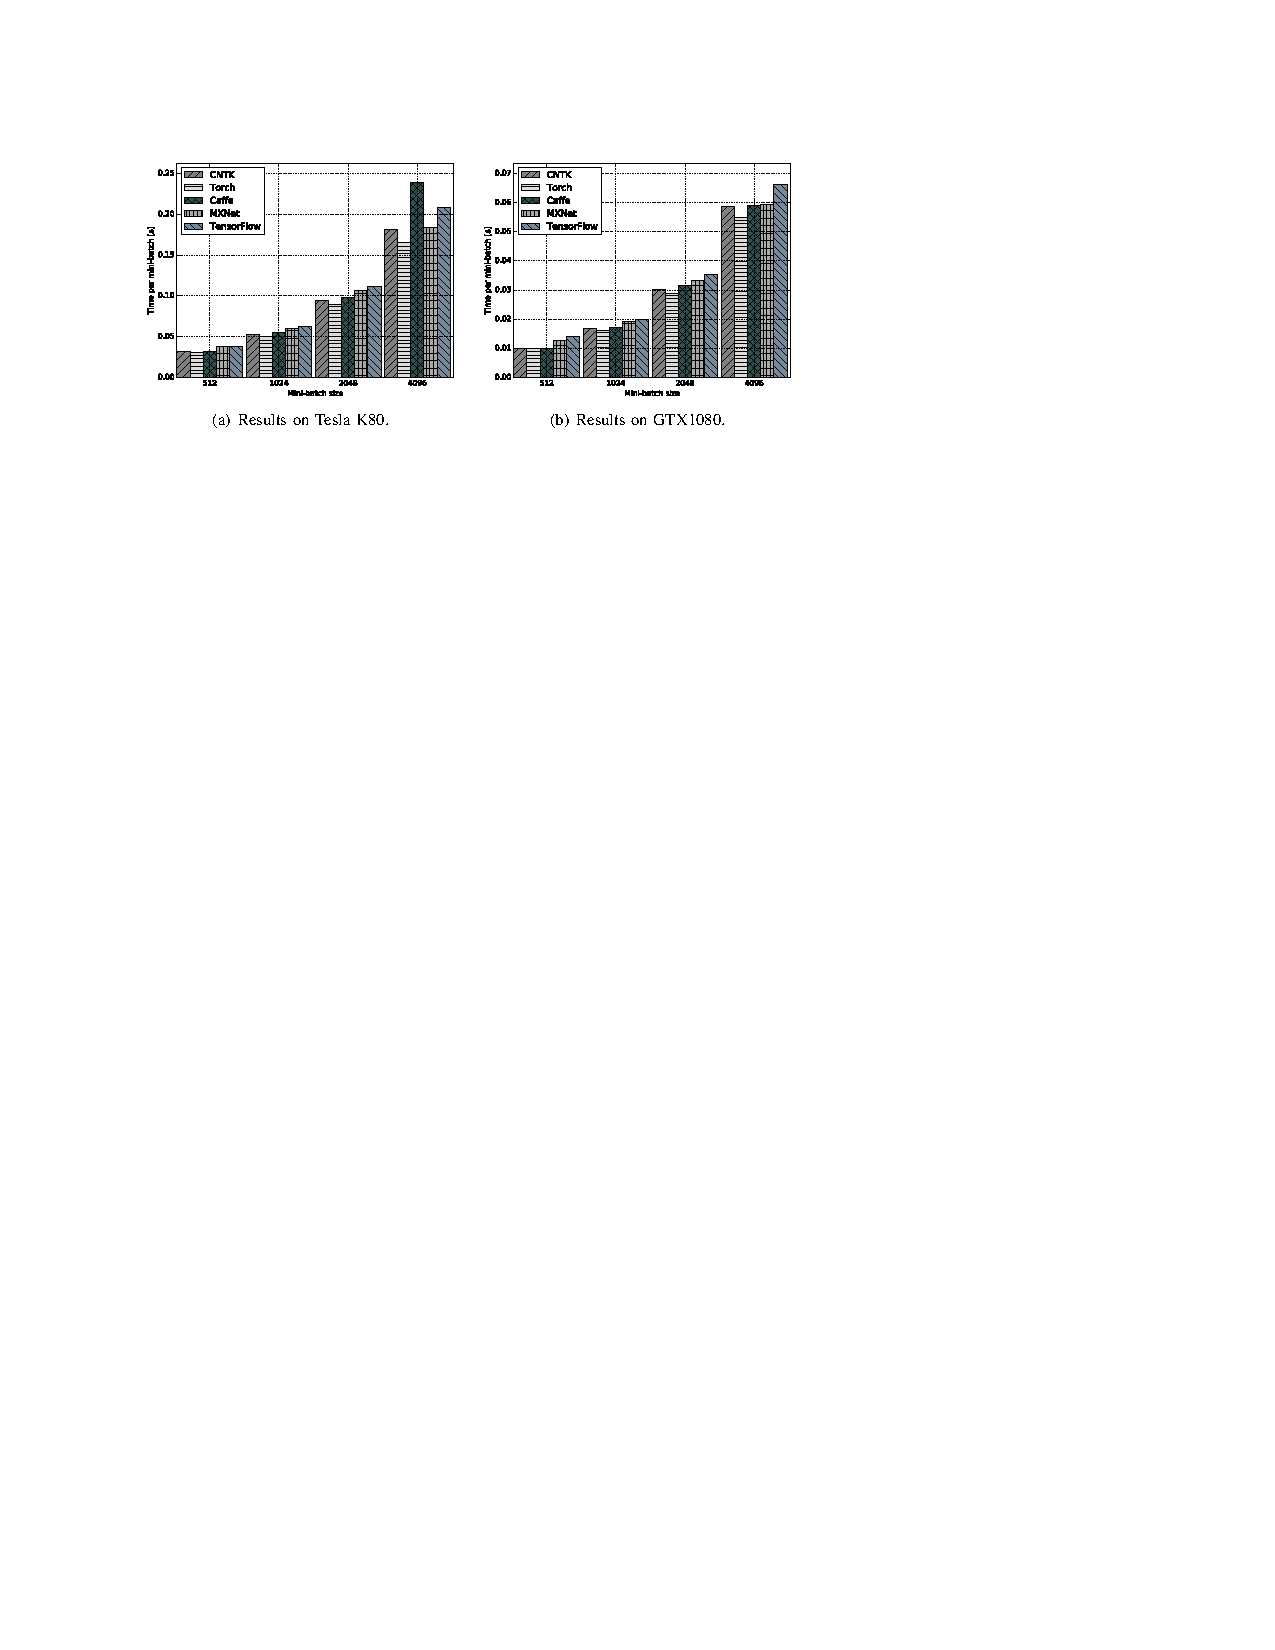
\includegraphics[height=1.8in]{figures/FCN-R2.pdf} 
		\caption{The performance comparison of FCN-R on GPU platforms.}
	\end{figure}
\end{frame}

%

\begin{frame}
	\MyLogo
	\frametitle{Numerical tests}  
	\begin{figure}[htbp] 
		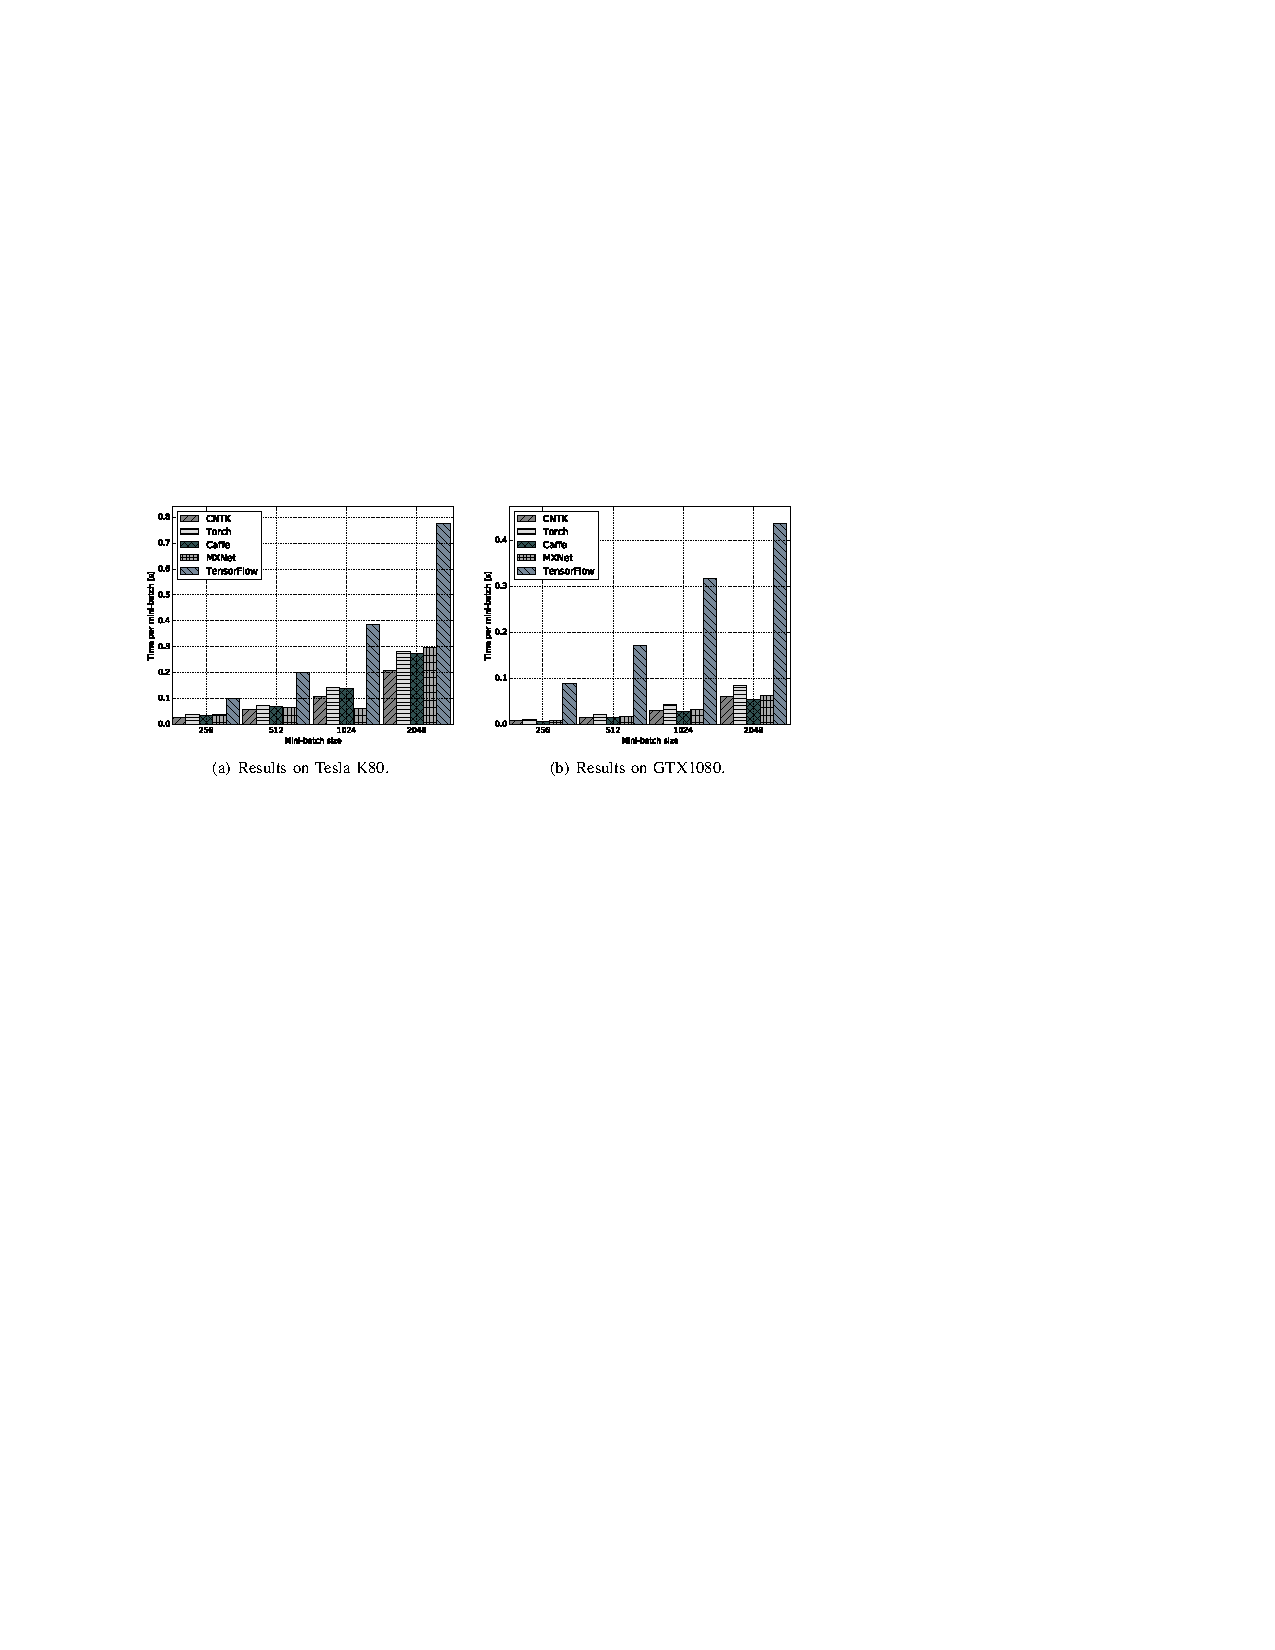
\includegraphics[height=1.8in]{figures/AlexNet-R2.pdf} 
		\caption{The performance comparison of AlexNet-R on GPU platforms.}
	\end{figure}
\end{frame}

%

\begin{frame}
	\MyLogo
	\frametitle{Numerical tests}  
	\begin{figure}[htbp] 
		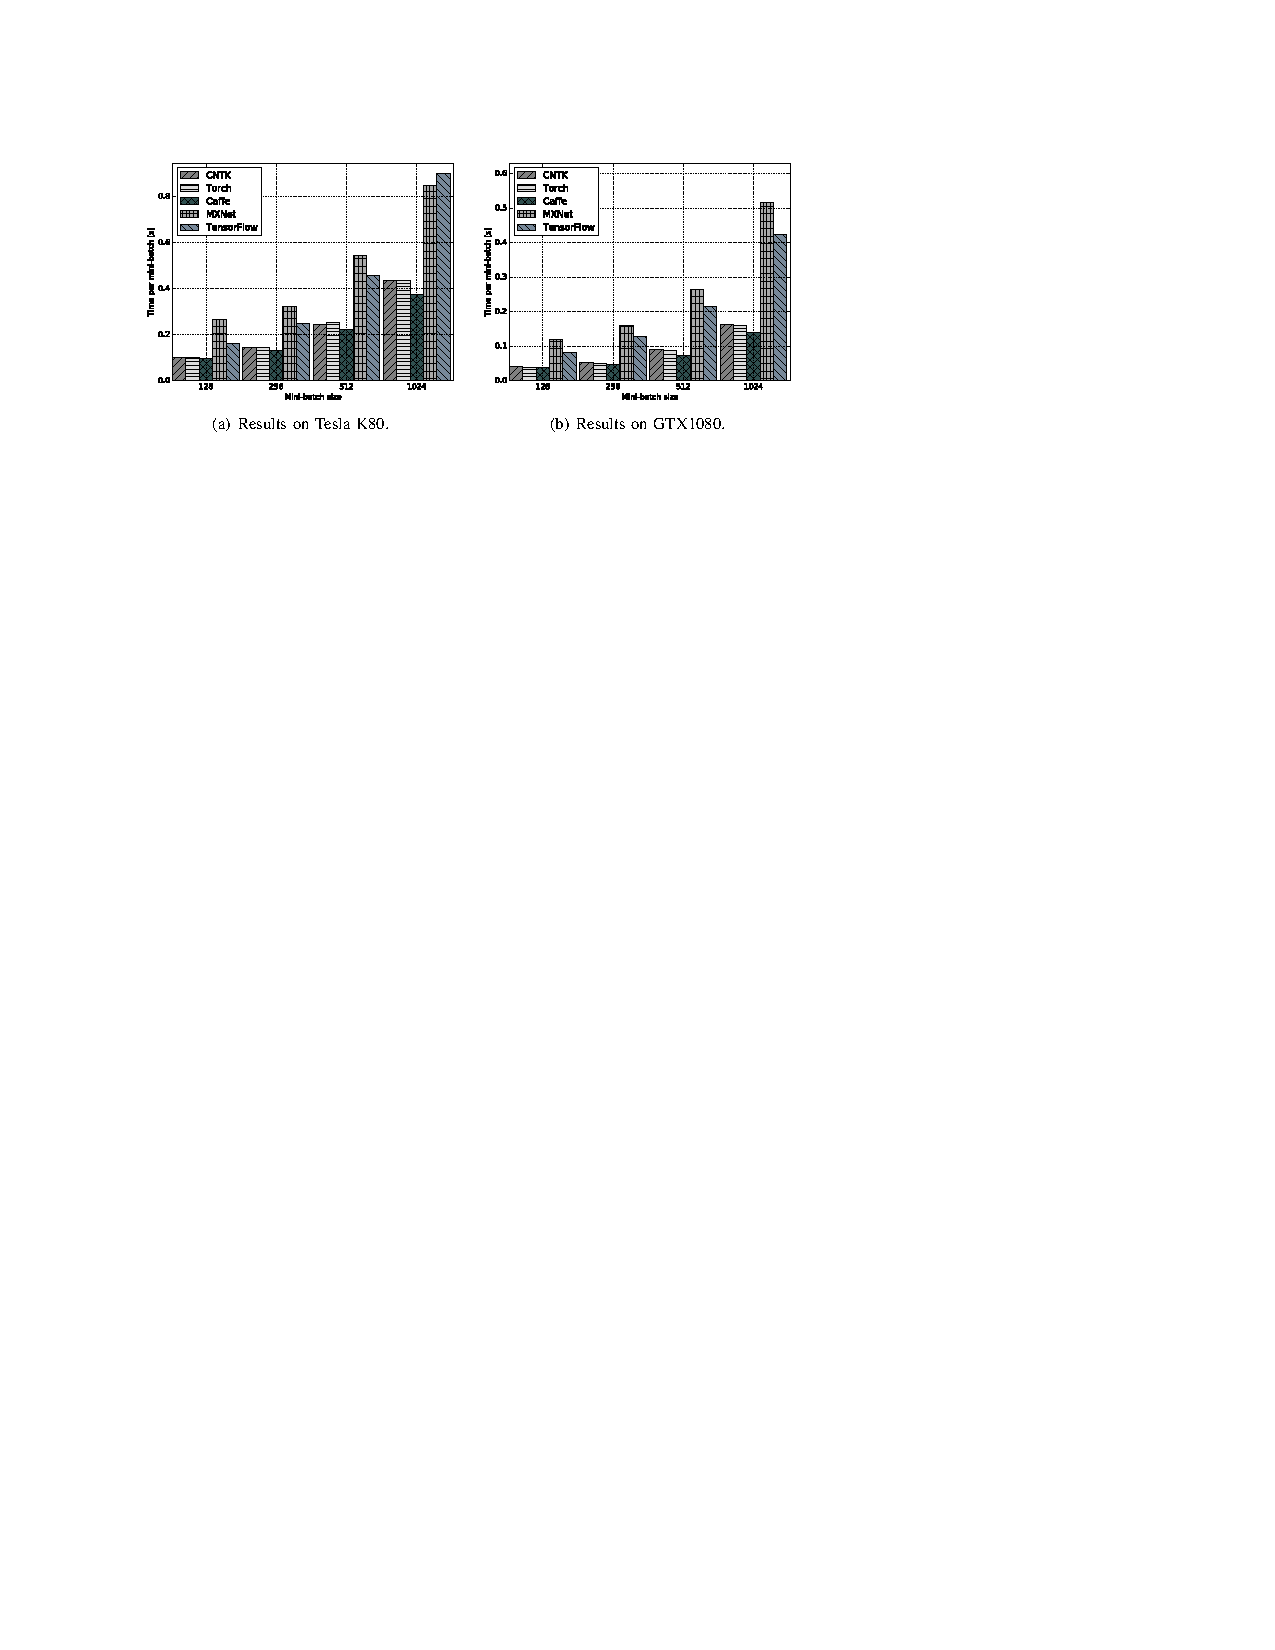
\includegraphics[height=1.8in]{figures/FCN-S2.pdf} 
		\caption{The performance comparison of FCN-S on GPU platforms.}
	\end{figure}
\end{frame}

%

\begin{frame}
	\MyLogo
	\frametitle{Numerical tests}  
	\begin{figure}[htbp] 
		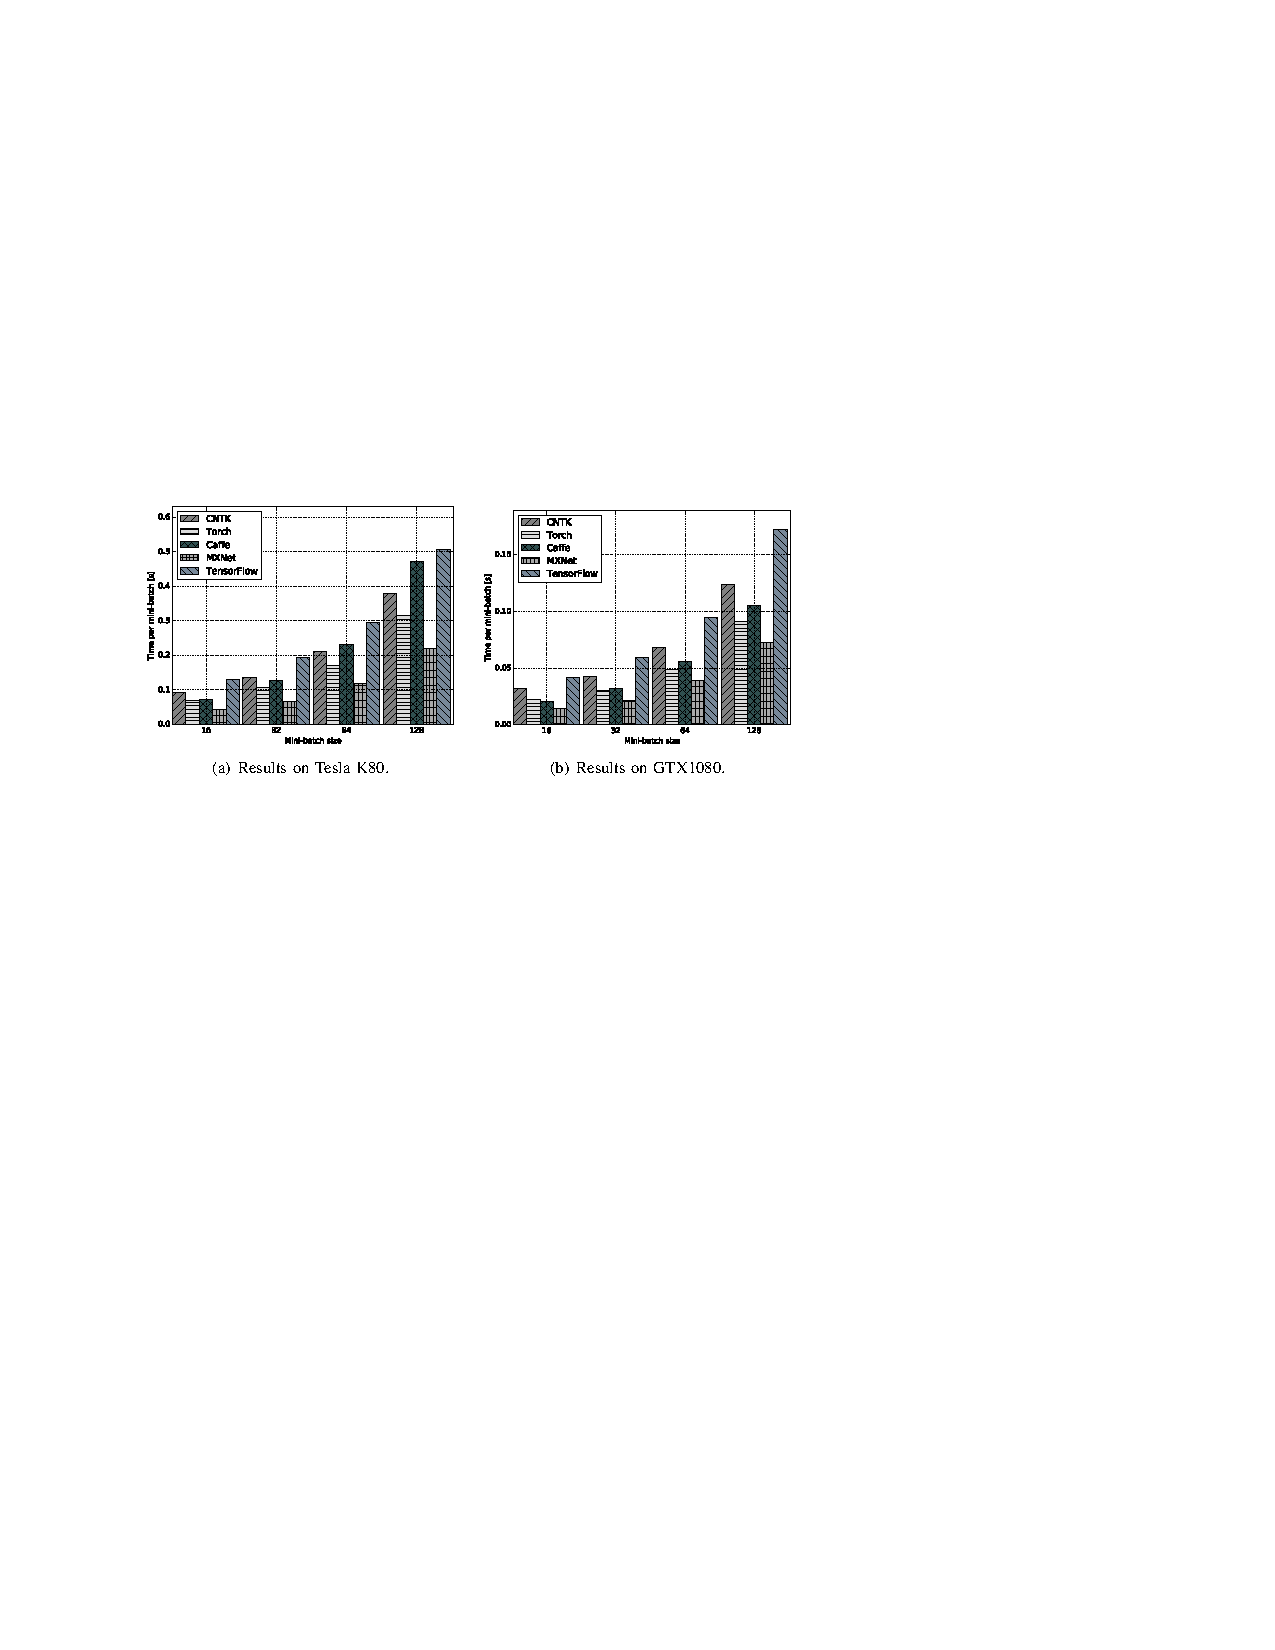
\includegraphics[height=1.8in]{figures/AlexNet-S2.pdf} 
		\caption{The performance comparison of AlexNet-S on GPU platforms.}
	\end{figure}
\end{frame}